\section{Durchführung}
\label{sec:Durchführung}
Zu erst muss der Versuchaufbau wie im Kapitel \ref{sec:Theorie} geschildert
aufgebaut werden. Die Apparatur ist in Abbildung \ref{fig:aufbau} zusehen.
Dann wird in die Reservoirs 3\si{\liter} Wasser eingefüllt. Eine Messreihe wird
damit gestartet, indem der Kompressor und die Rührmotoren angestellt werden und
sofort die beide Temperaturen,die Drücke $p_a$ und $p_b$ sowie
die Leistungsaufnahme des Kompressors notiert.
Im Tonus von 1 Minute werden nun die zuvor genannten Werte notiert. Die Messreihe wird
abgebrochen, wenn $T_1 = 50 \si{\celsius}$.
\begin{figure}
  \centering
  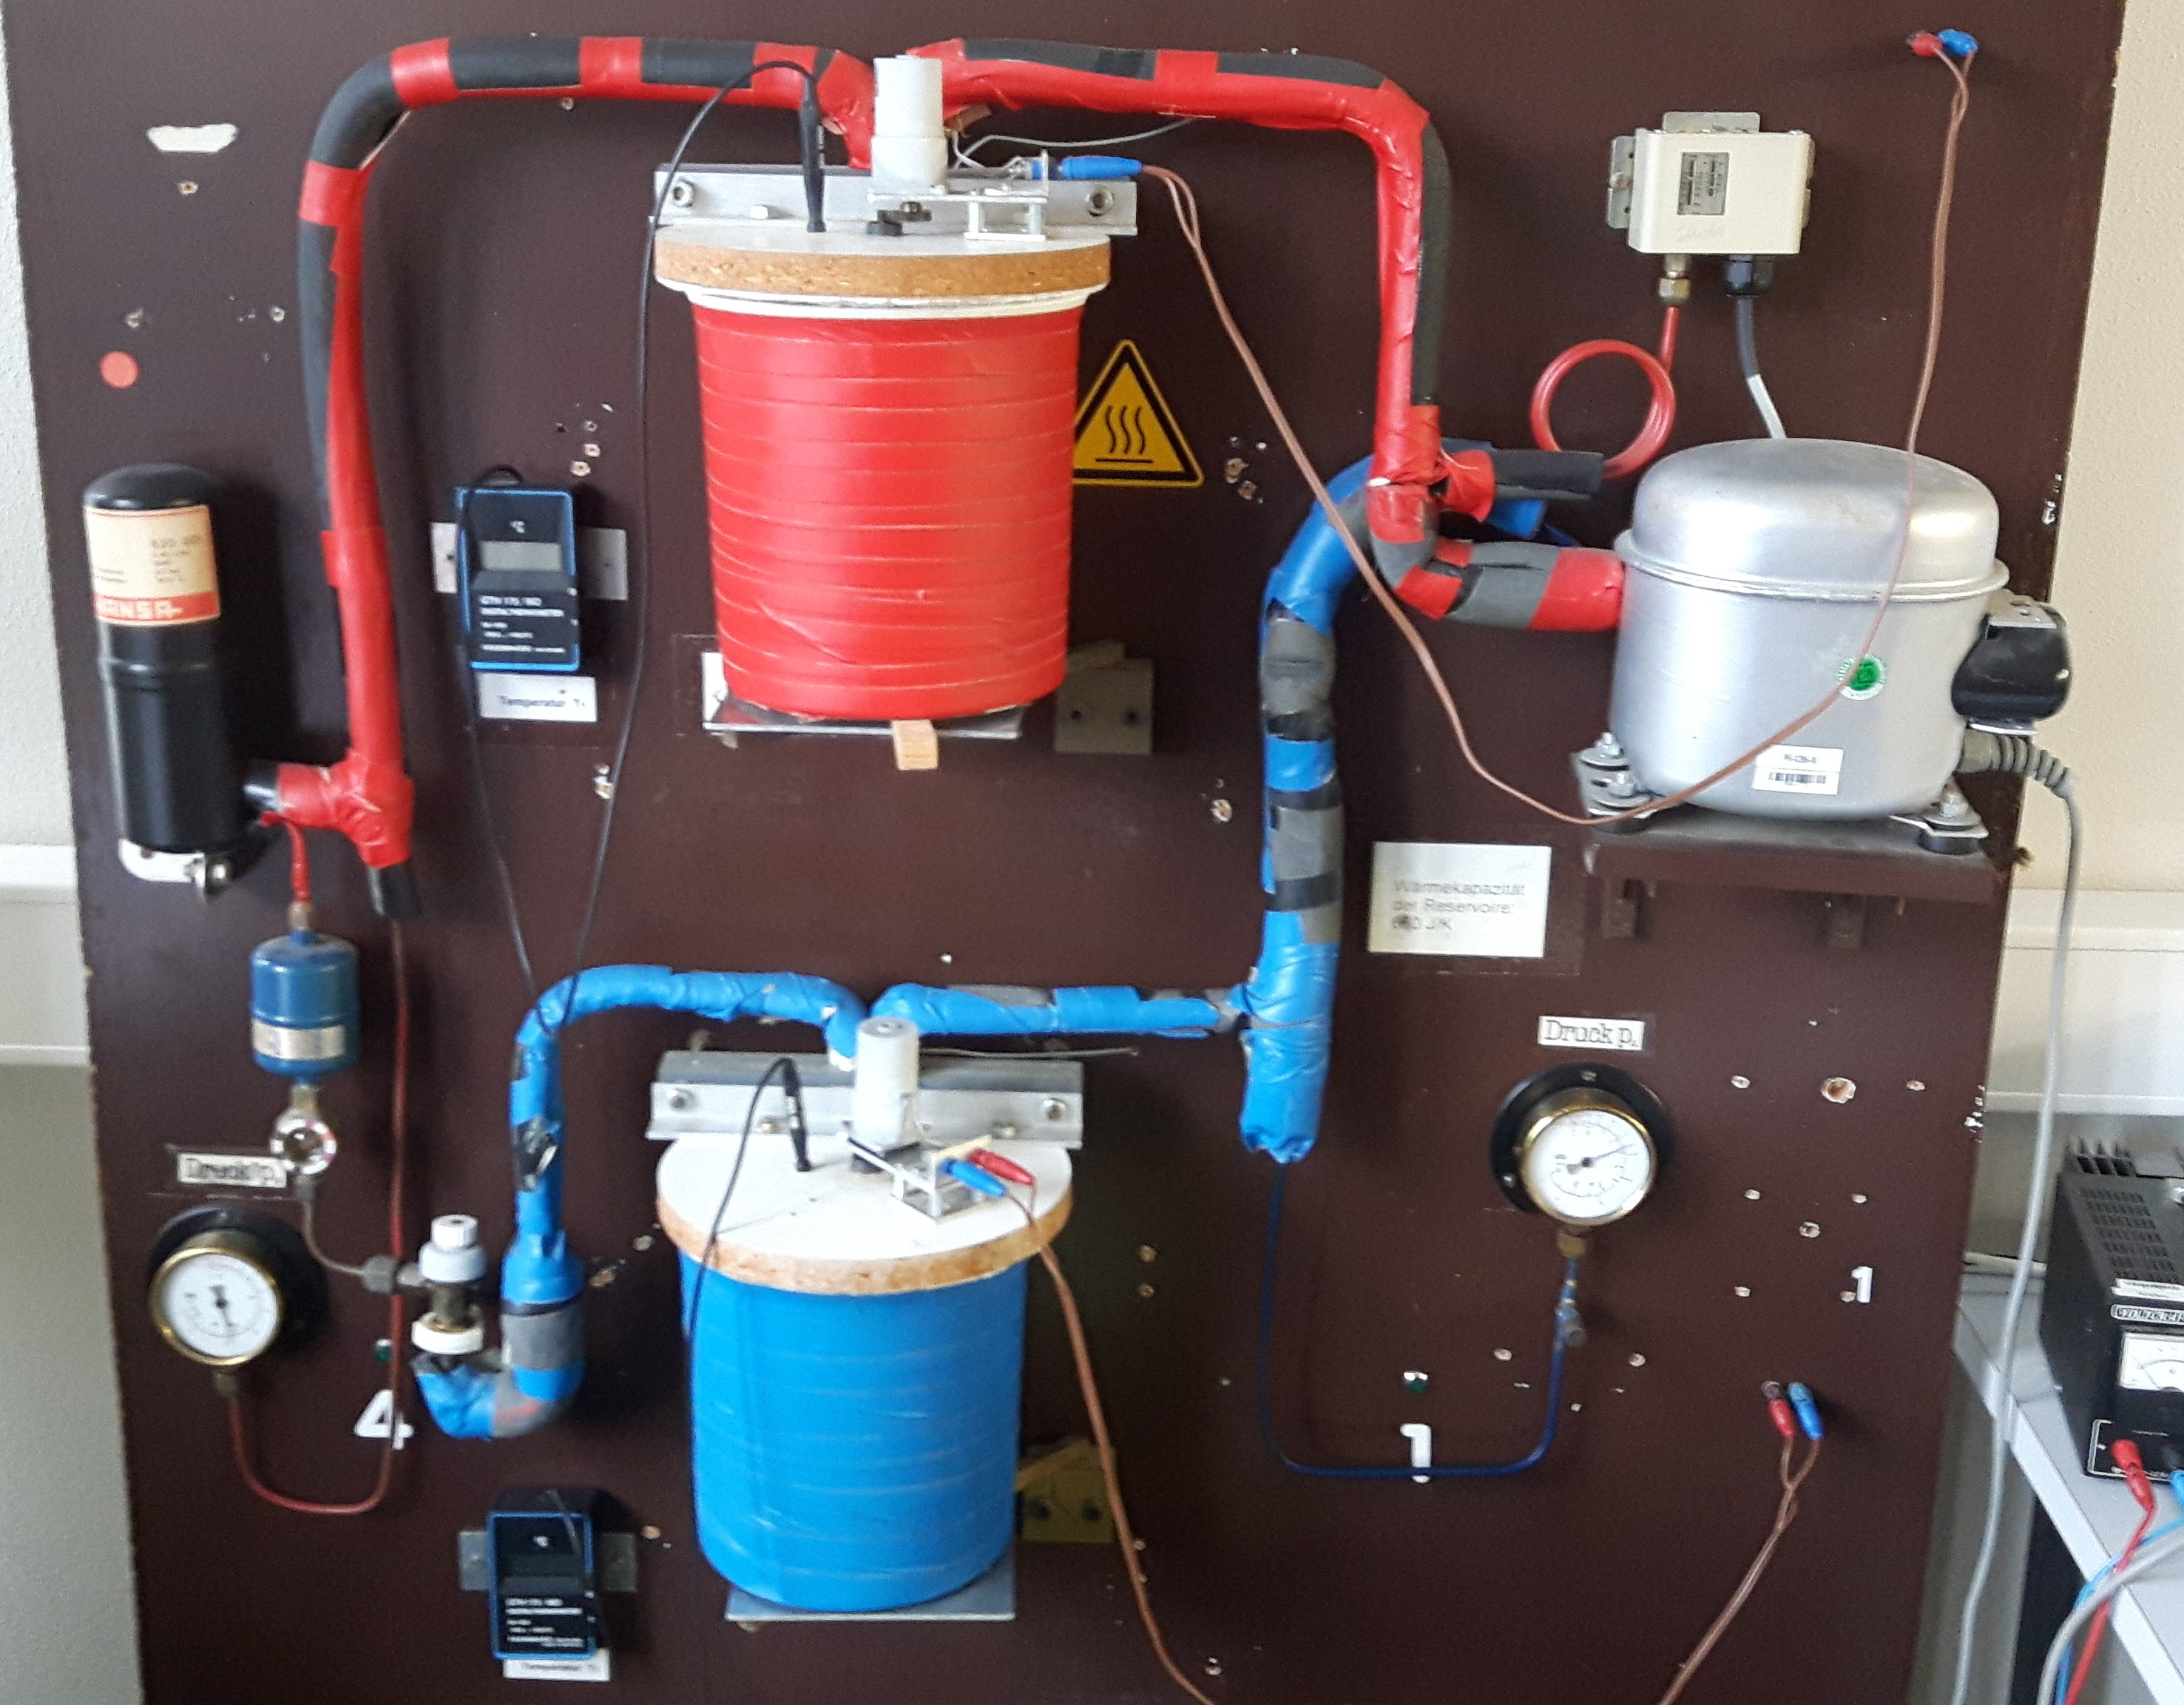
\includegraphics[height = 7cm]{logos/realAufbau.jpg}
  \caption{Versuchs Aufbau}
  \label{fig:aufbau}
\end{figure}
